
\chapter{Appendix}

\begin{figure}[ht]
       \centering 
	    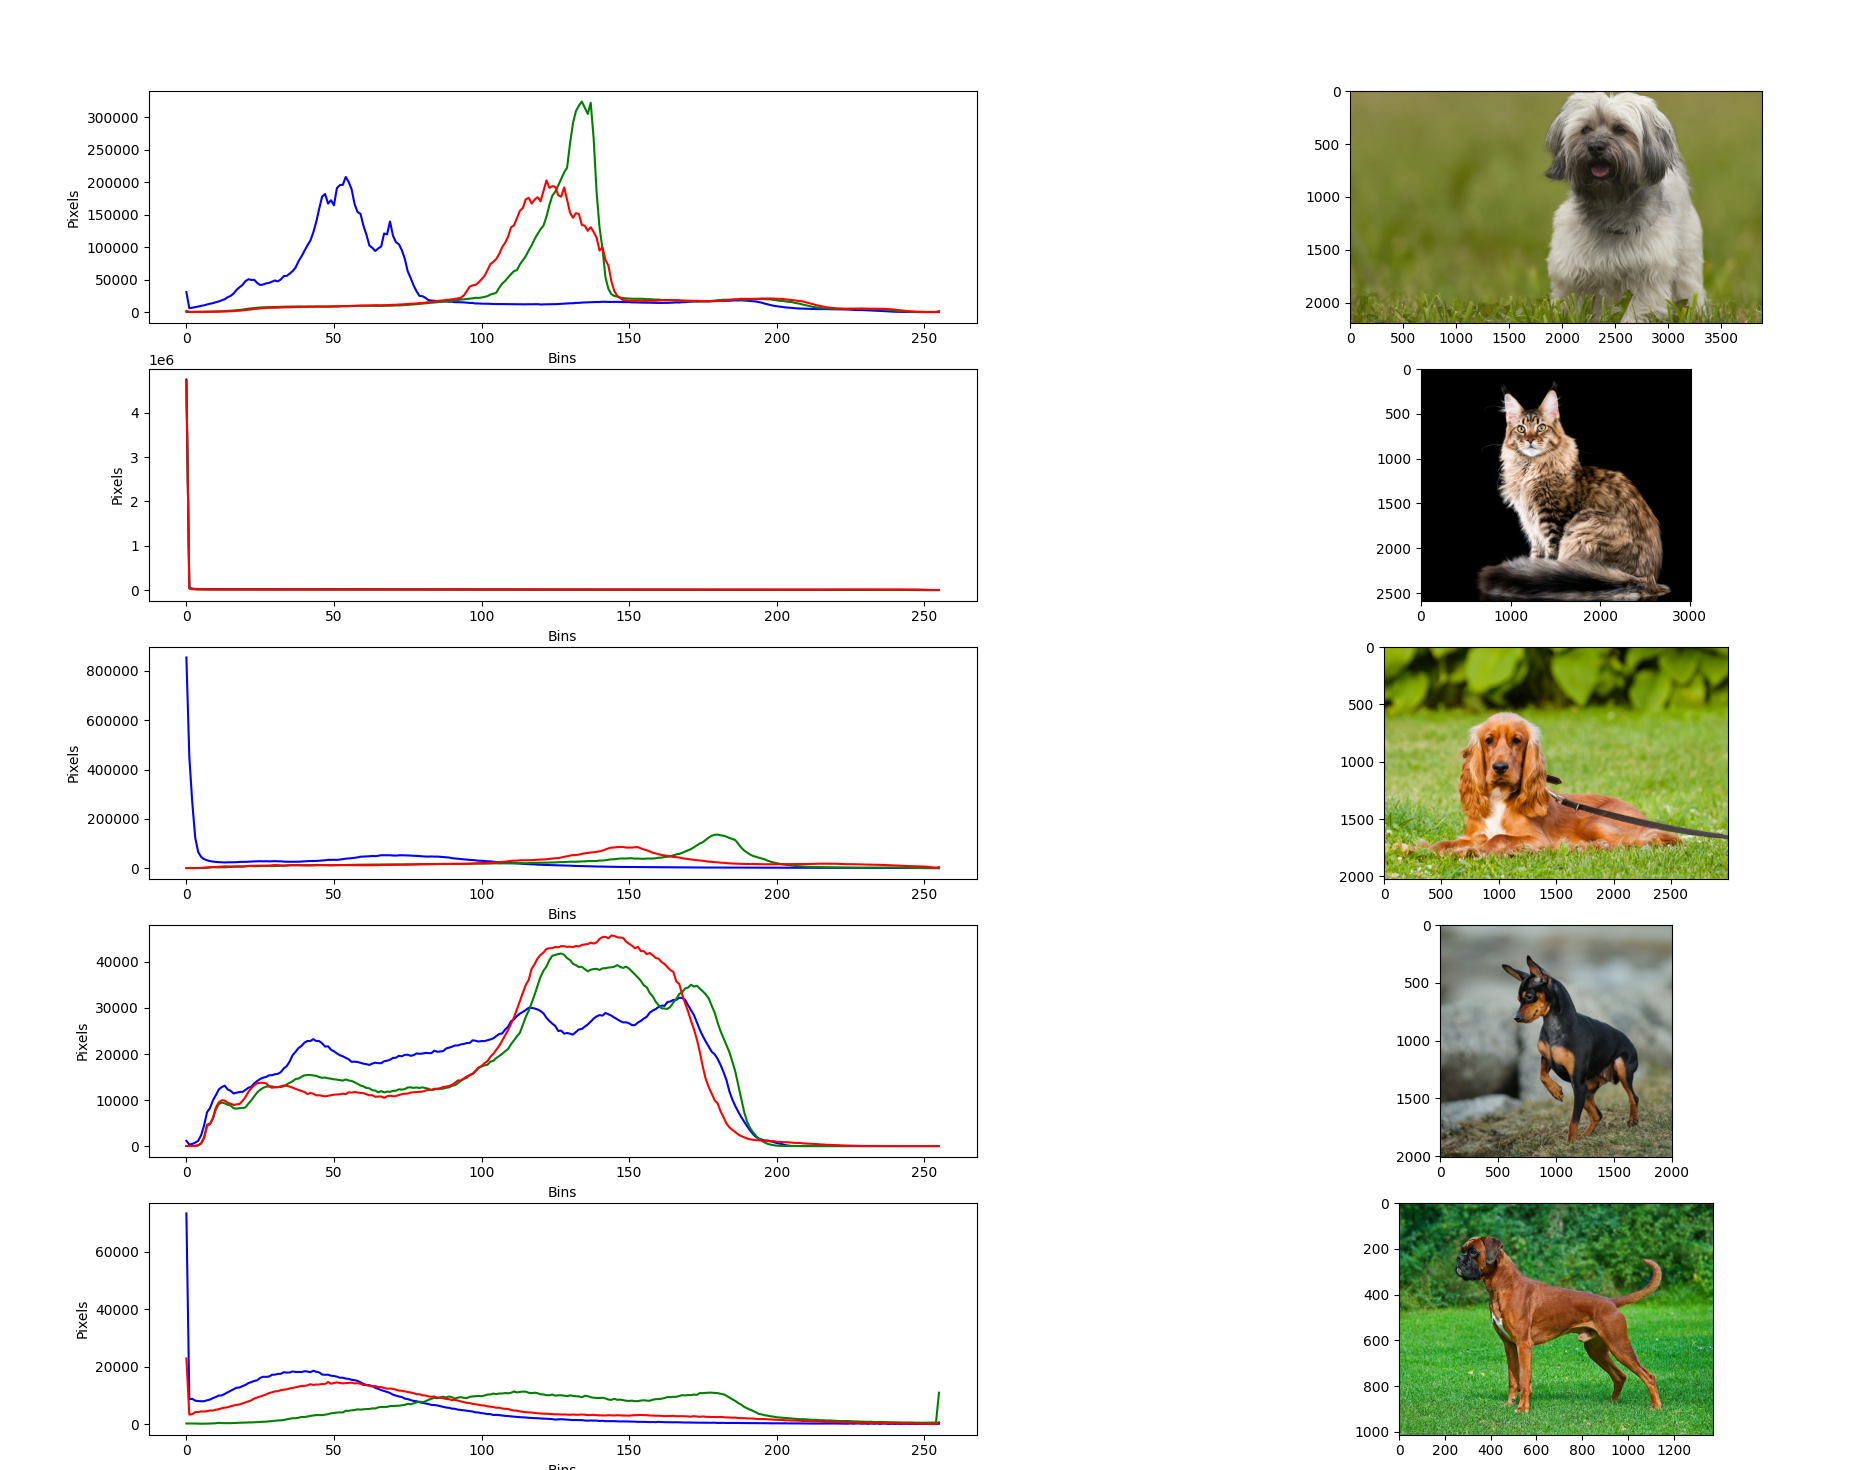
\includegraphics[width = 13 cm]{slowest_files_vgg.png}
        \caption{Histogram of the slowest files in common amongst all models}
         \label{fig:slowest_files_all}
\end{figure}

\begin{figure}[ht]
       \centering 
	    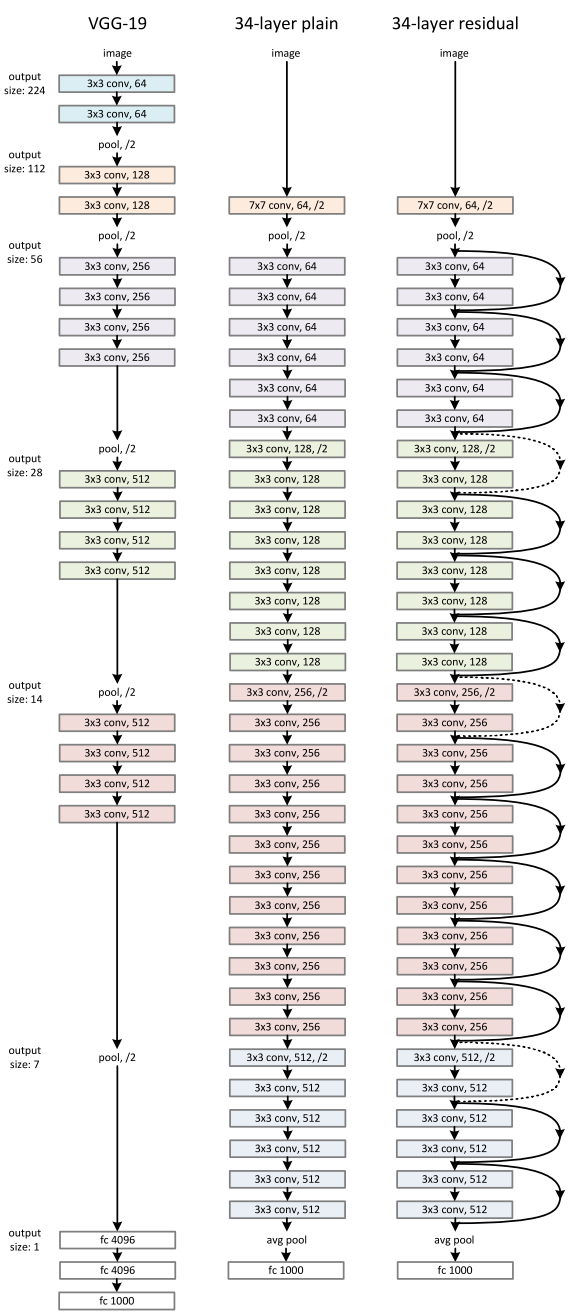
\includegraphics[width = 10 cm]{resnet_arch_full.png}
        \caption[Example of the architecture of residual networks]{ Left: the VGG-19 model [41] (19.6 billion FLOPs) as a reference. Middle: a plain network with 34 parameter layers (3.6 billion FLOPs). Right: a residual network with 34 parameter layers (3.6 billion FLOPs). The dotted shortcuts increase dimensions.\cite{DBLP:journals/corr/HeZRS15}}
         \label{fig:resnet_arch_full}
\end{figure}
\begin{figure}[ht]
       \centering 
	    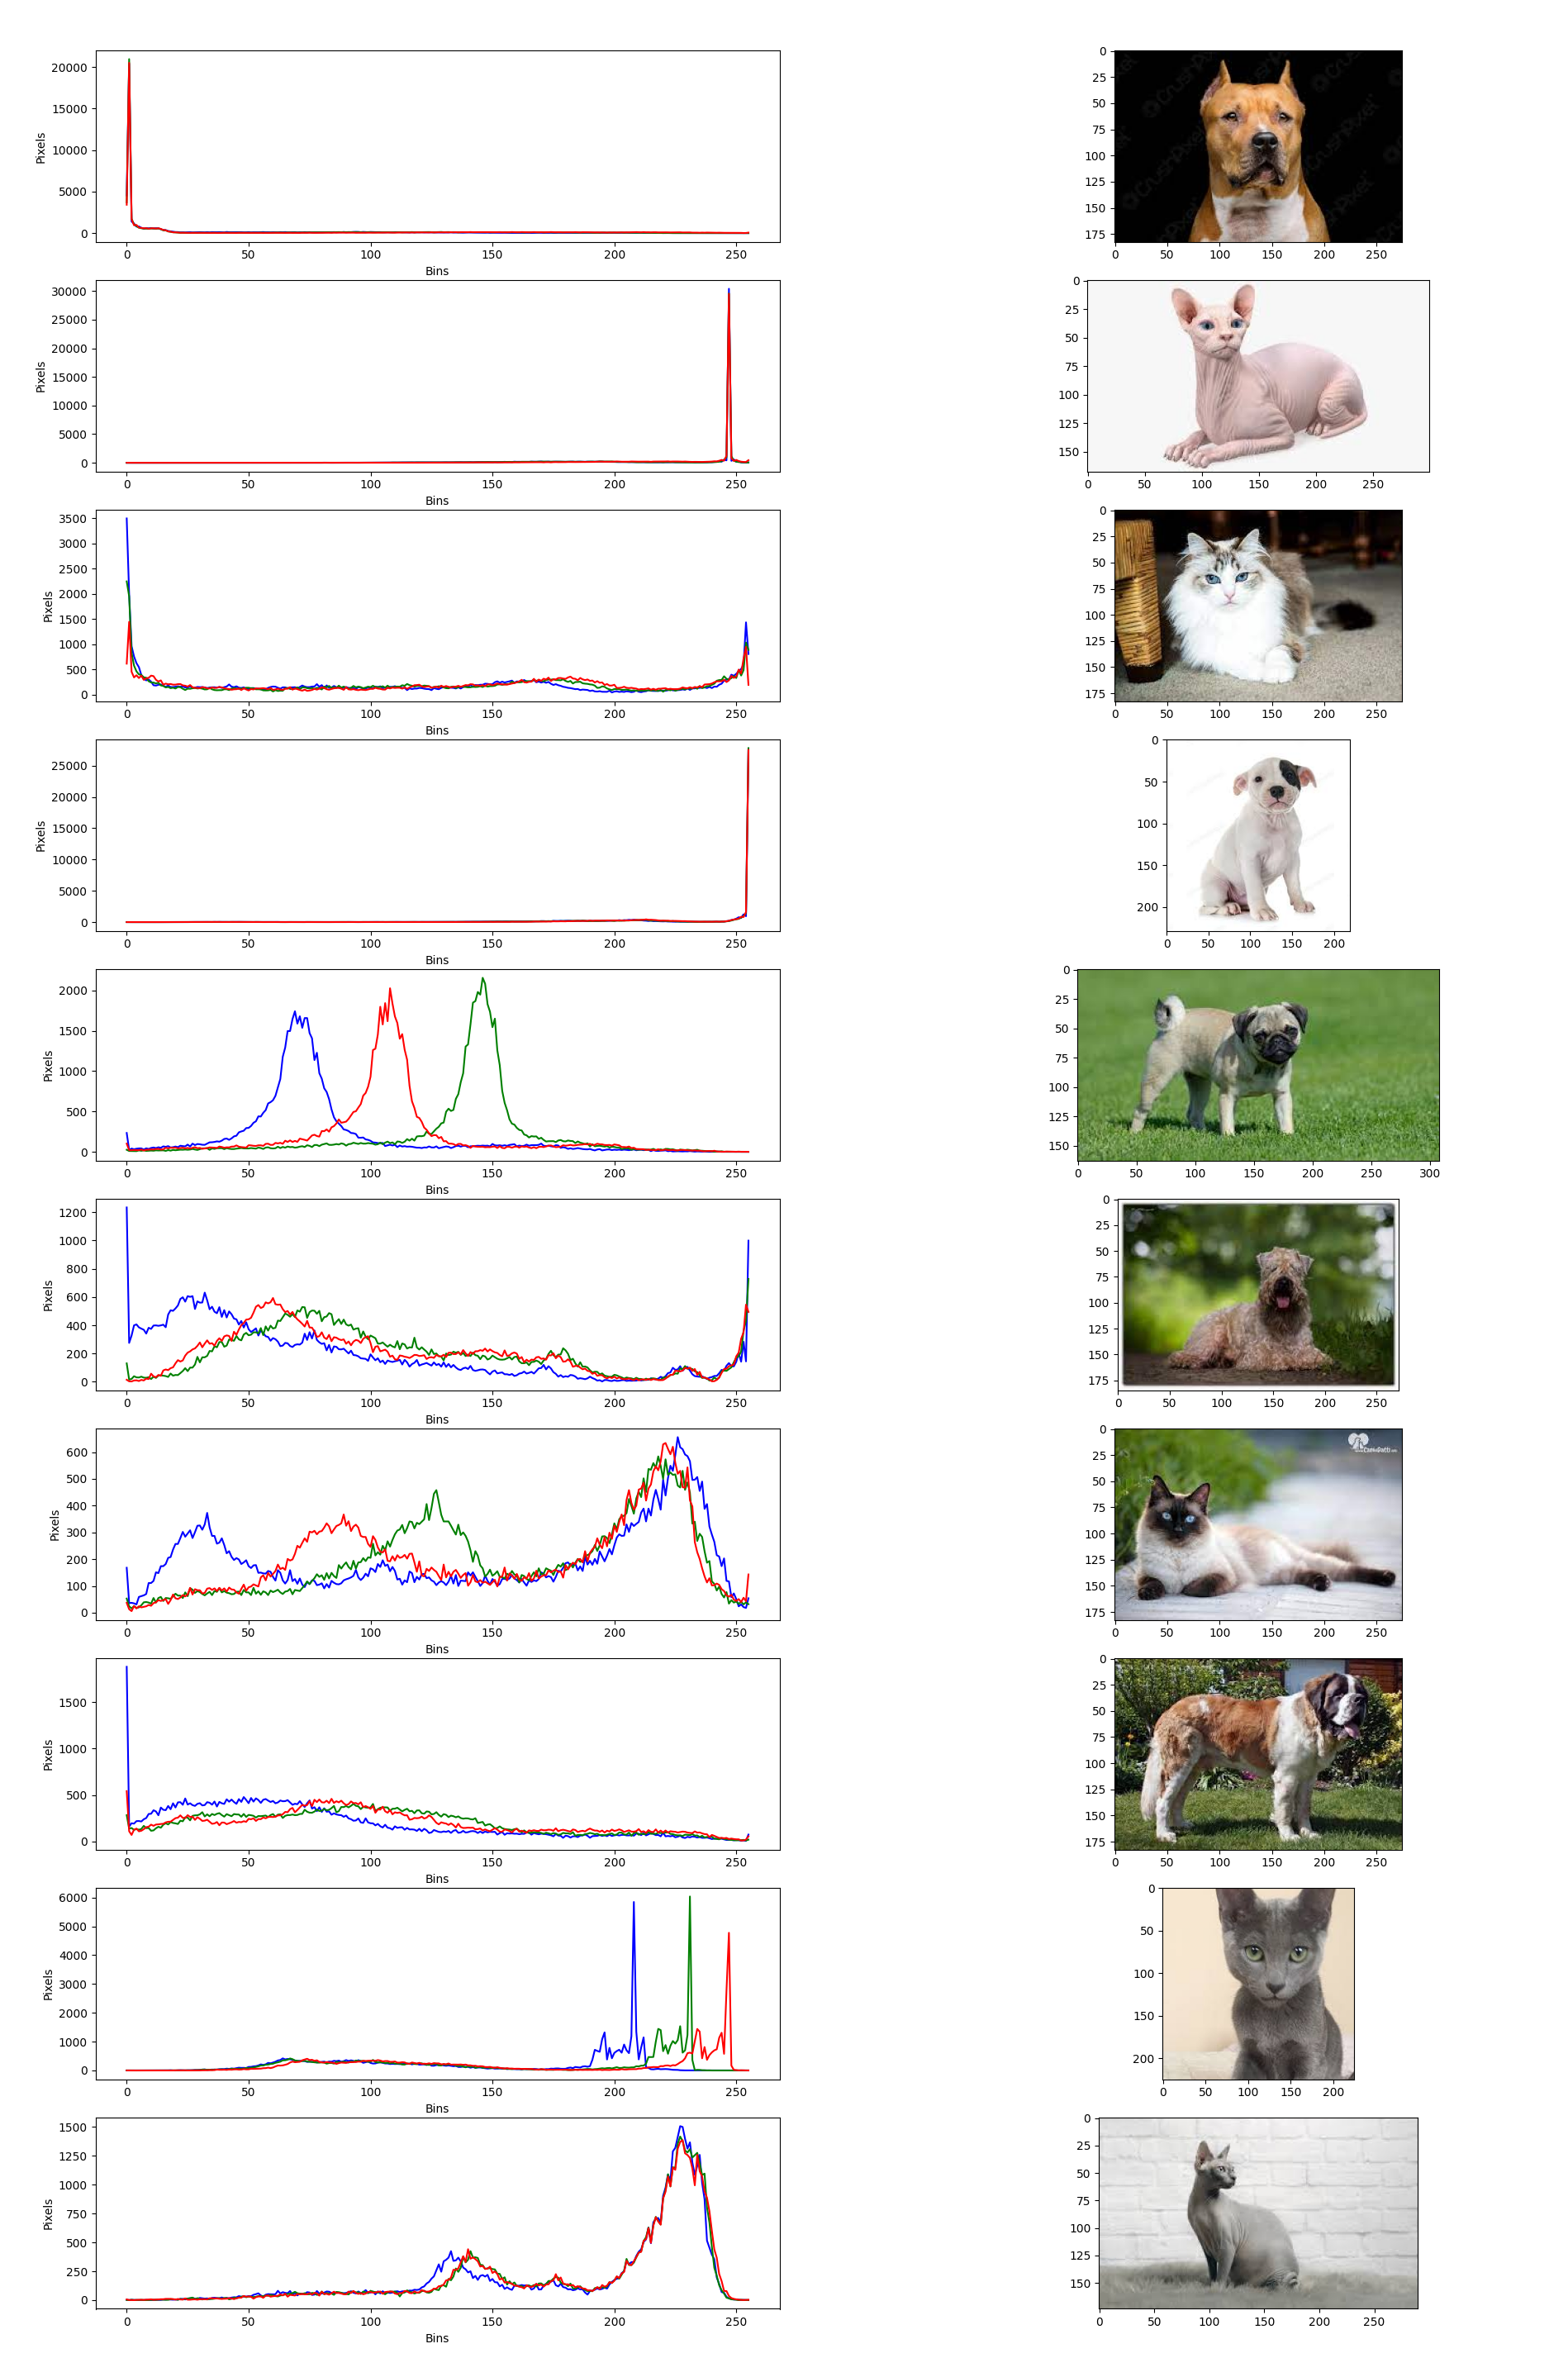
\includegraphics[width = 13 cm]{fastest_files.png}
        \caption{Histogram of the fastest files of Resnet 152}
         \label{fig:fastest_files_his}
\end{figure}

\begin{figure}[ht]
       \centering 
	    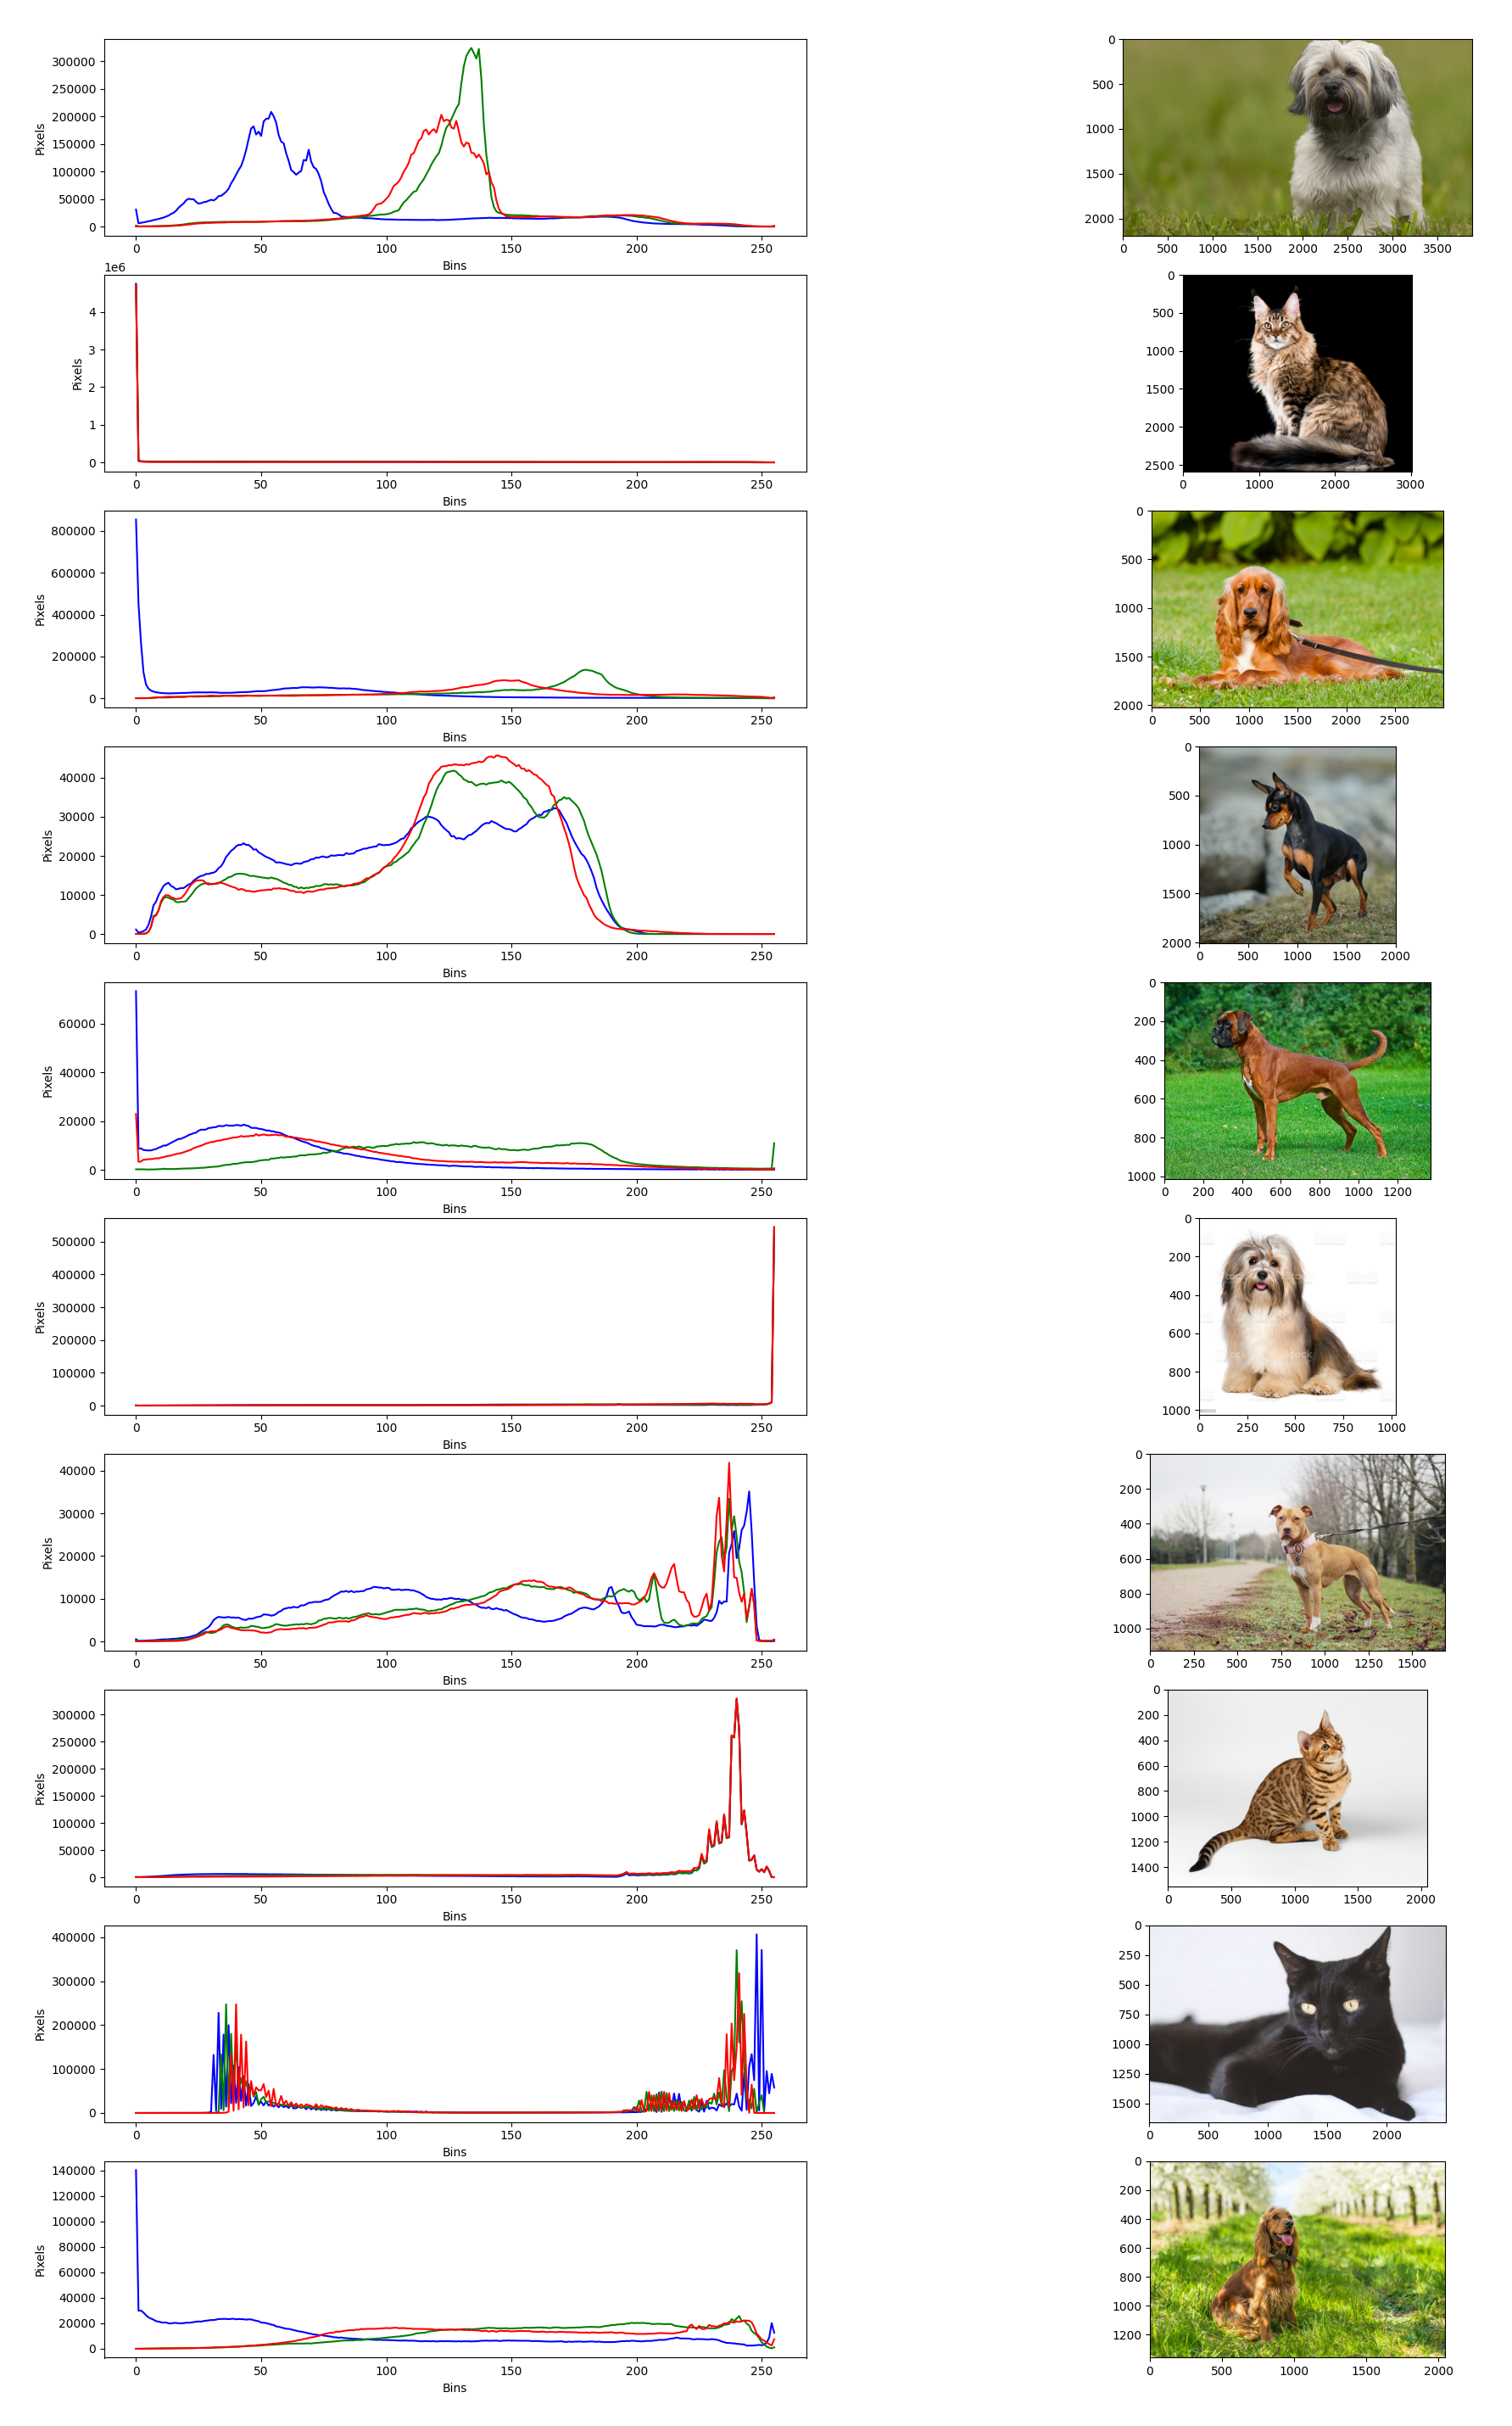
\includegraphics[width = 13 cm]{slowest_files.png}
        \caption{Histogram of the slowest files of Resnet152}
         \label{fig:slowest_files_his}
\end{figure}



\begin{figure}[ht]
       \centering 
	    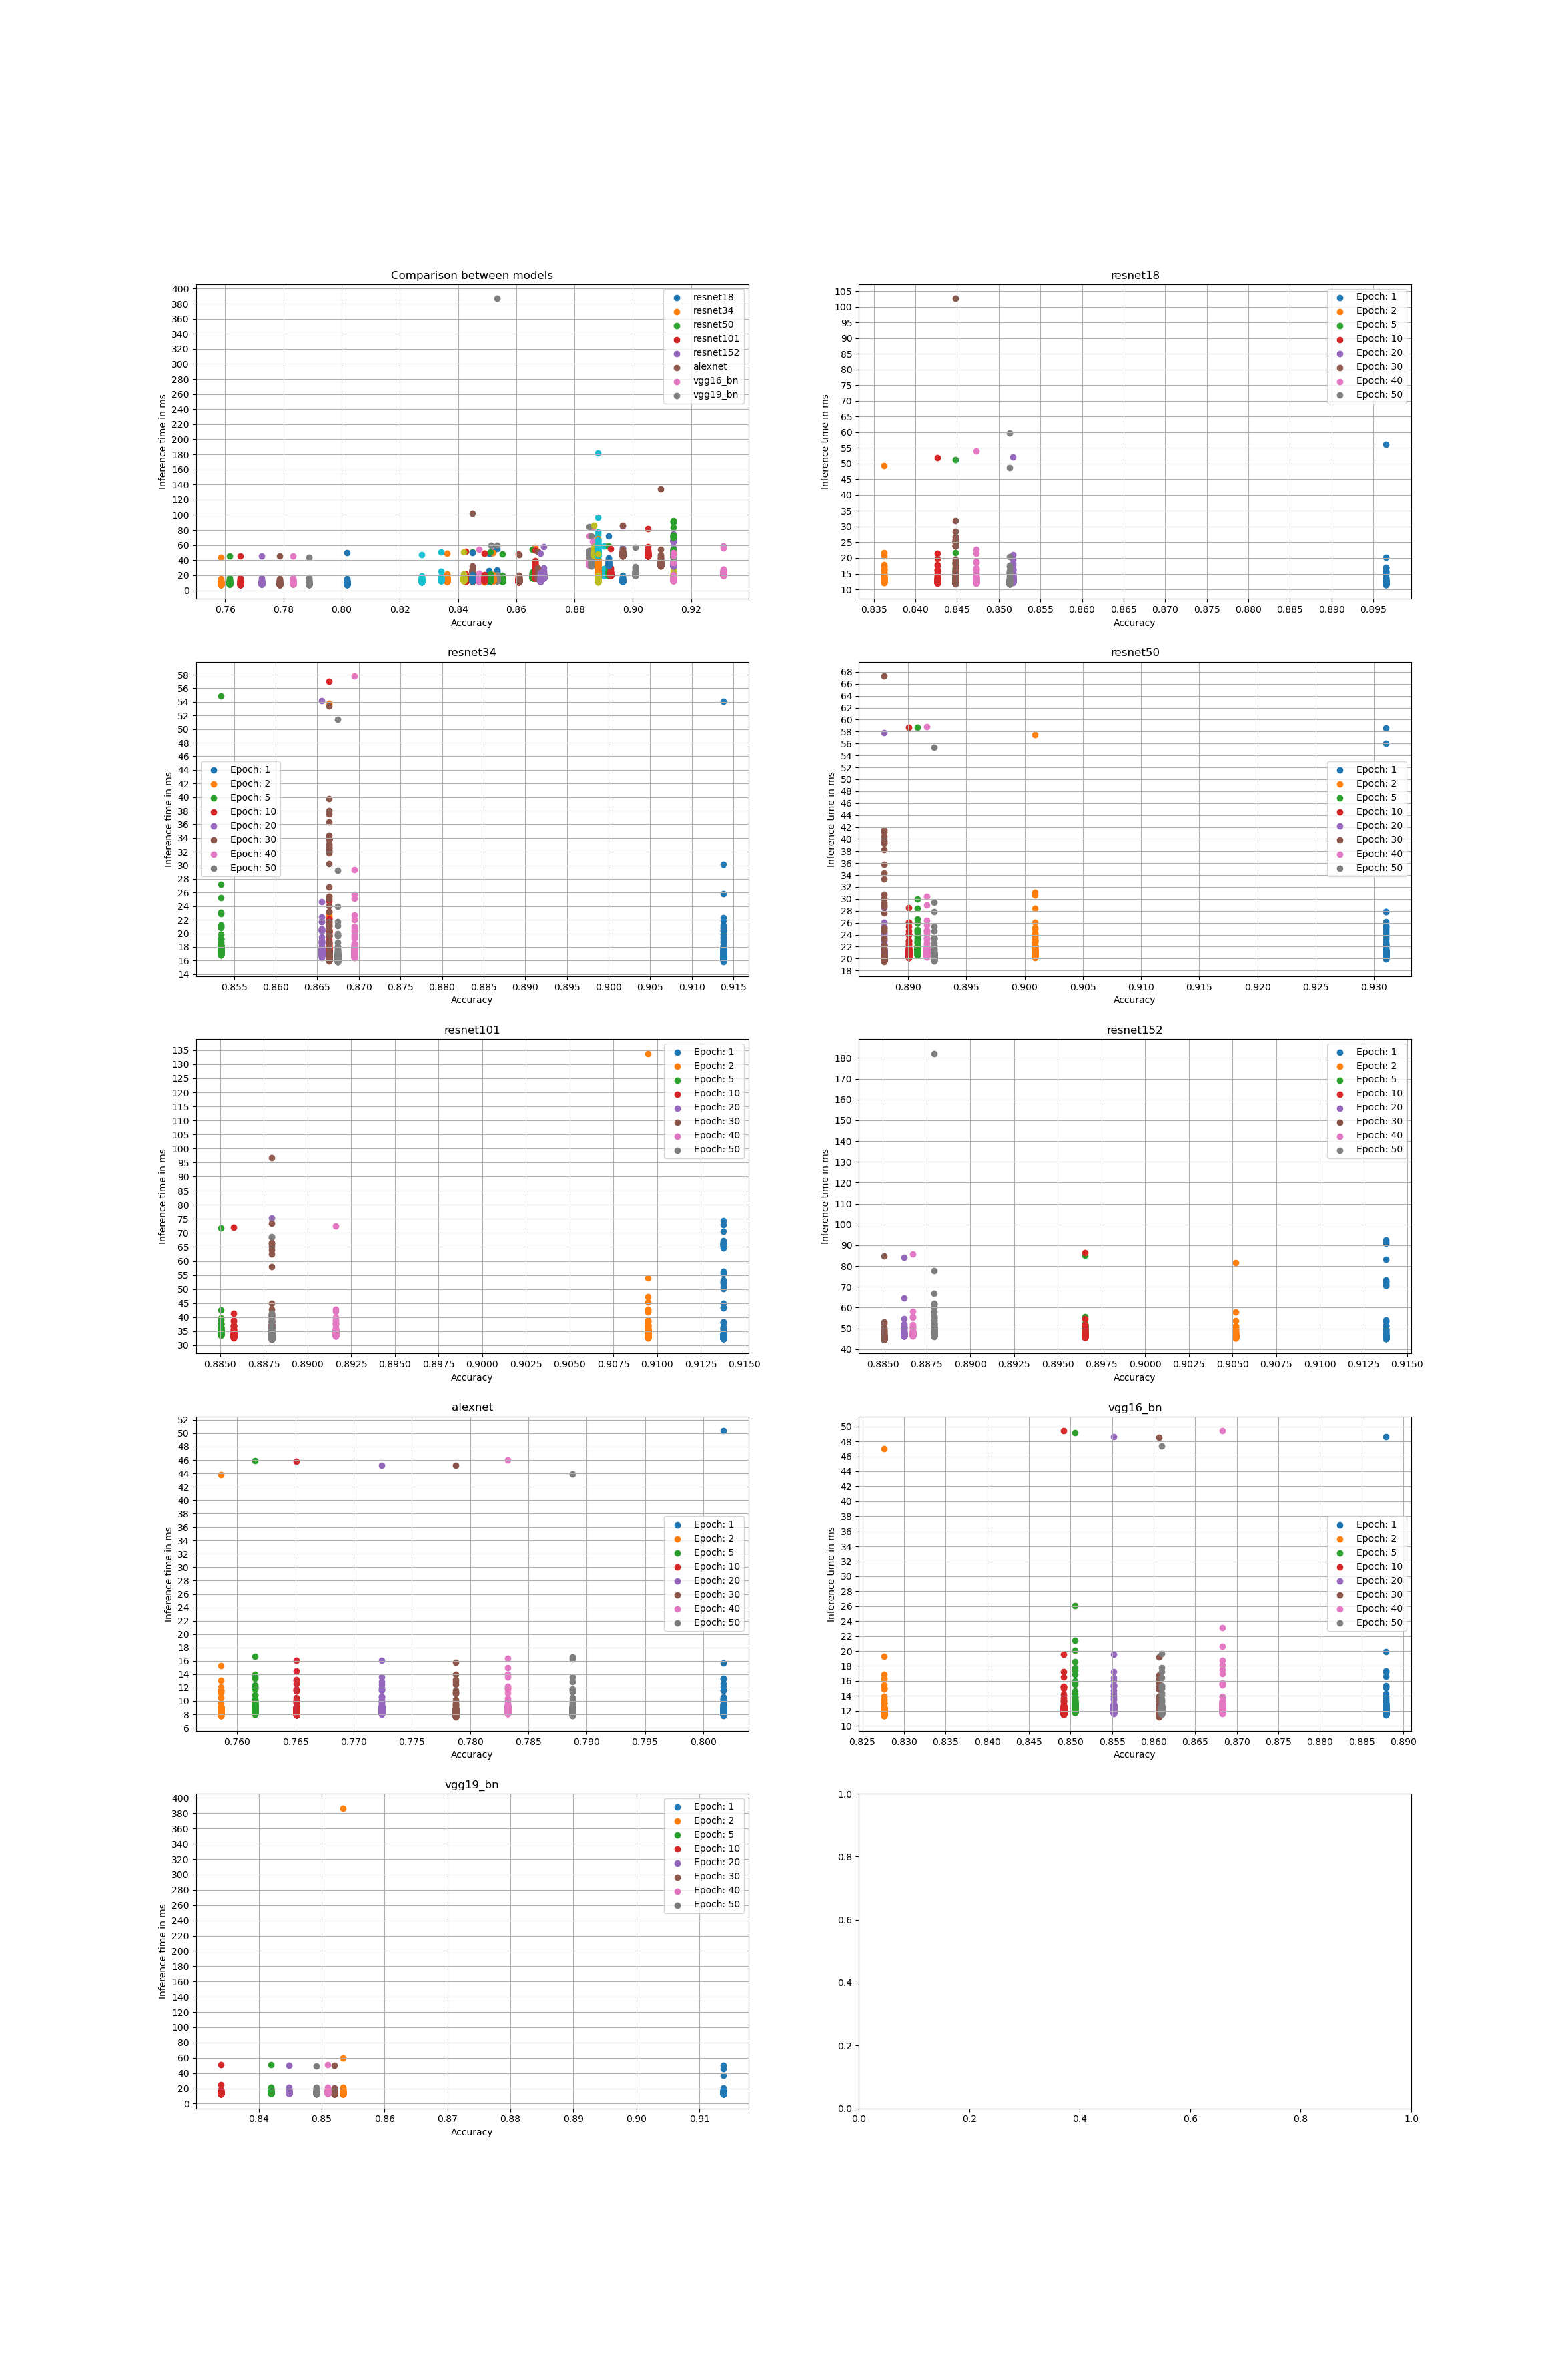
\includegraphics[width = 15 cm]{accuracy_inferencetime_seedlings.png}
        \caption{Complete result of the test for inference time in the seedlings dataset}
         \label{fig:accuracy_inferencetime_seedlings}
\end{figure}


\begin{figure}[ht]
       \centering 
	    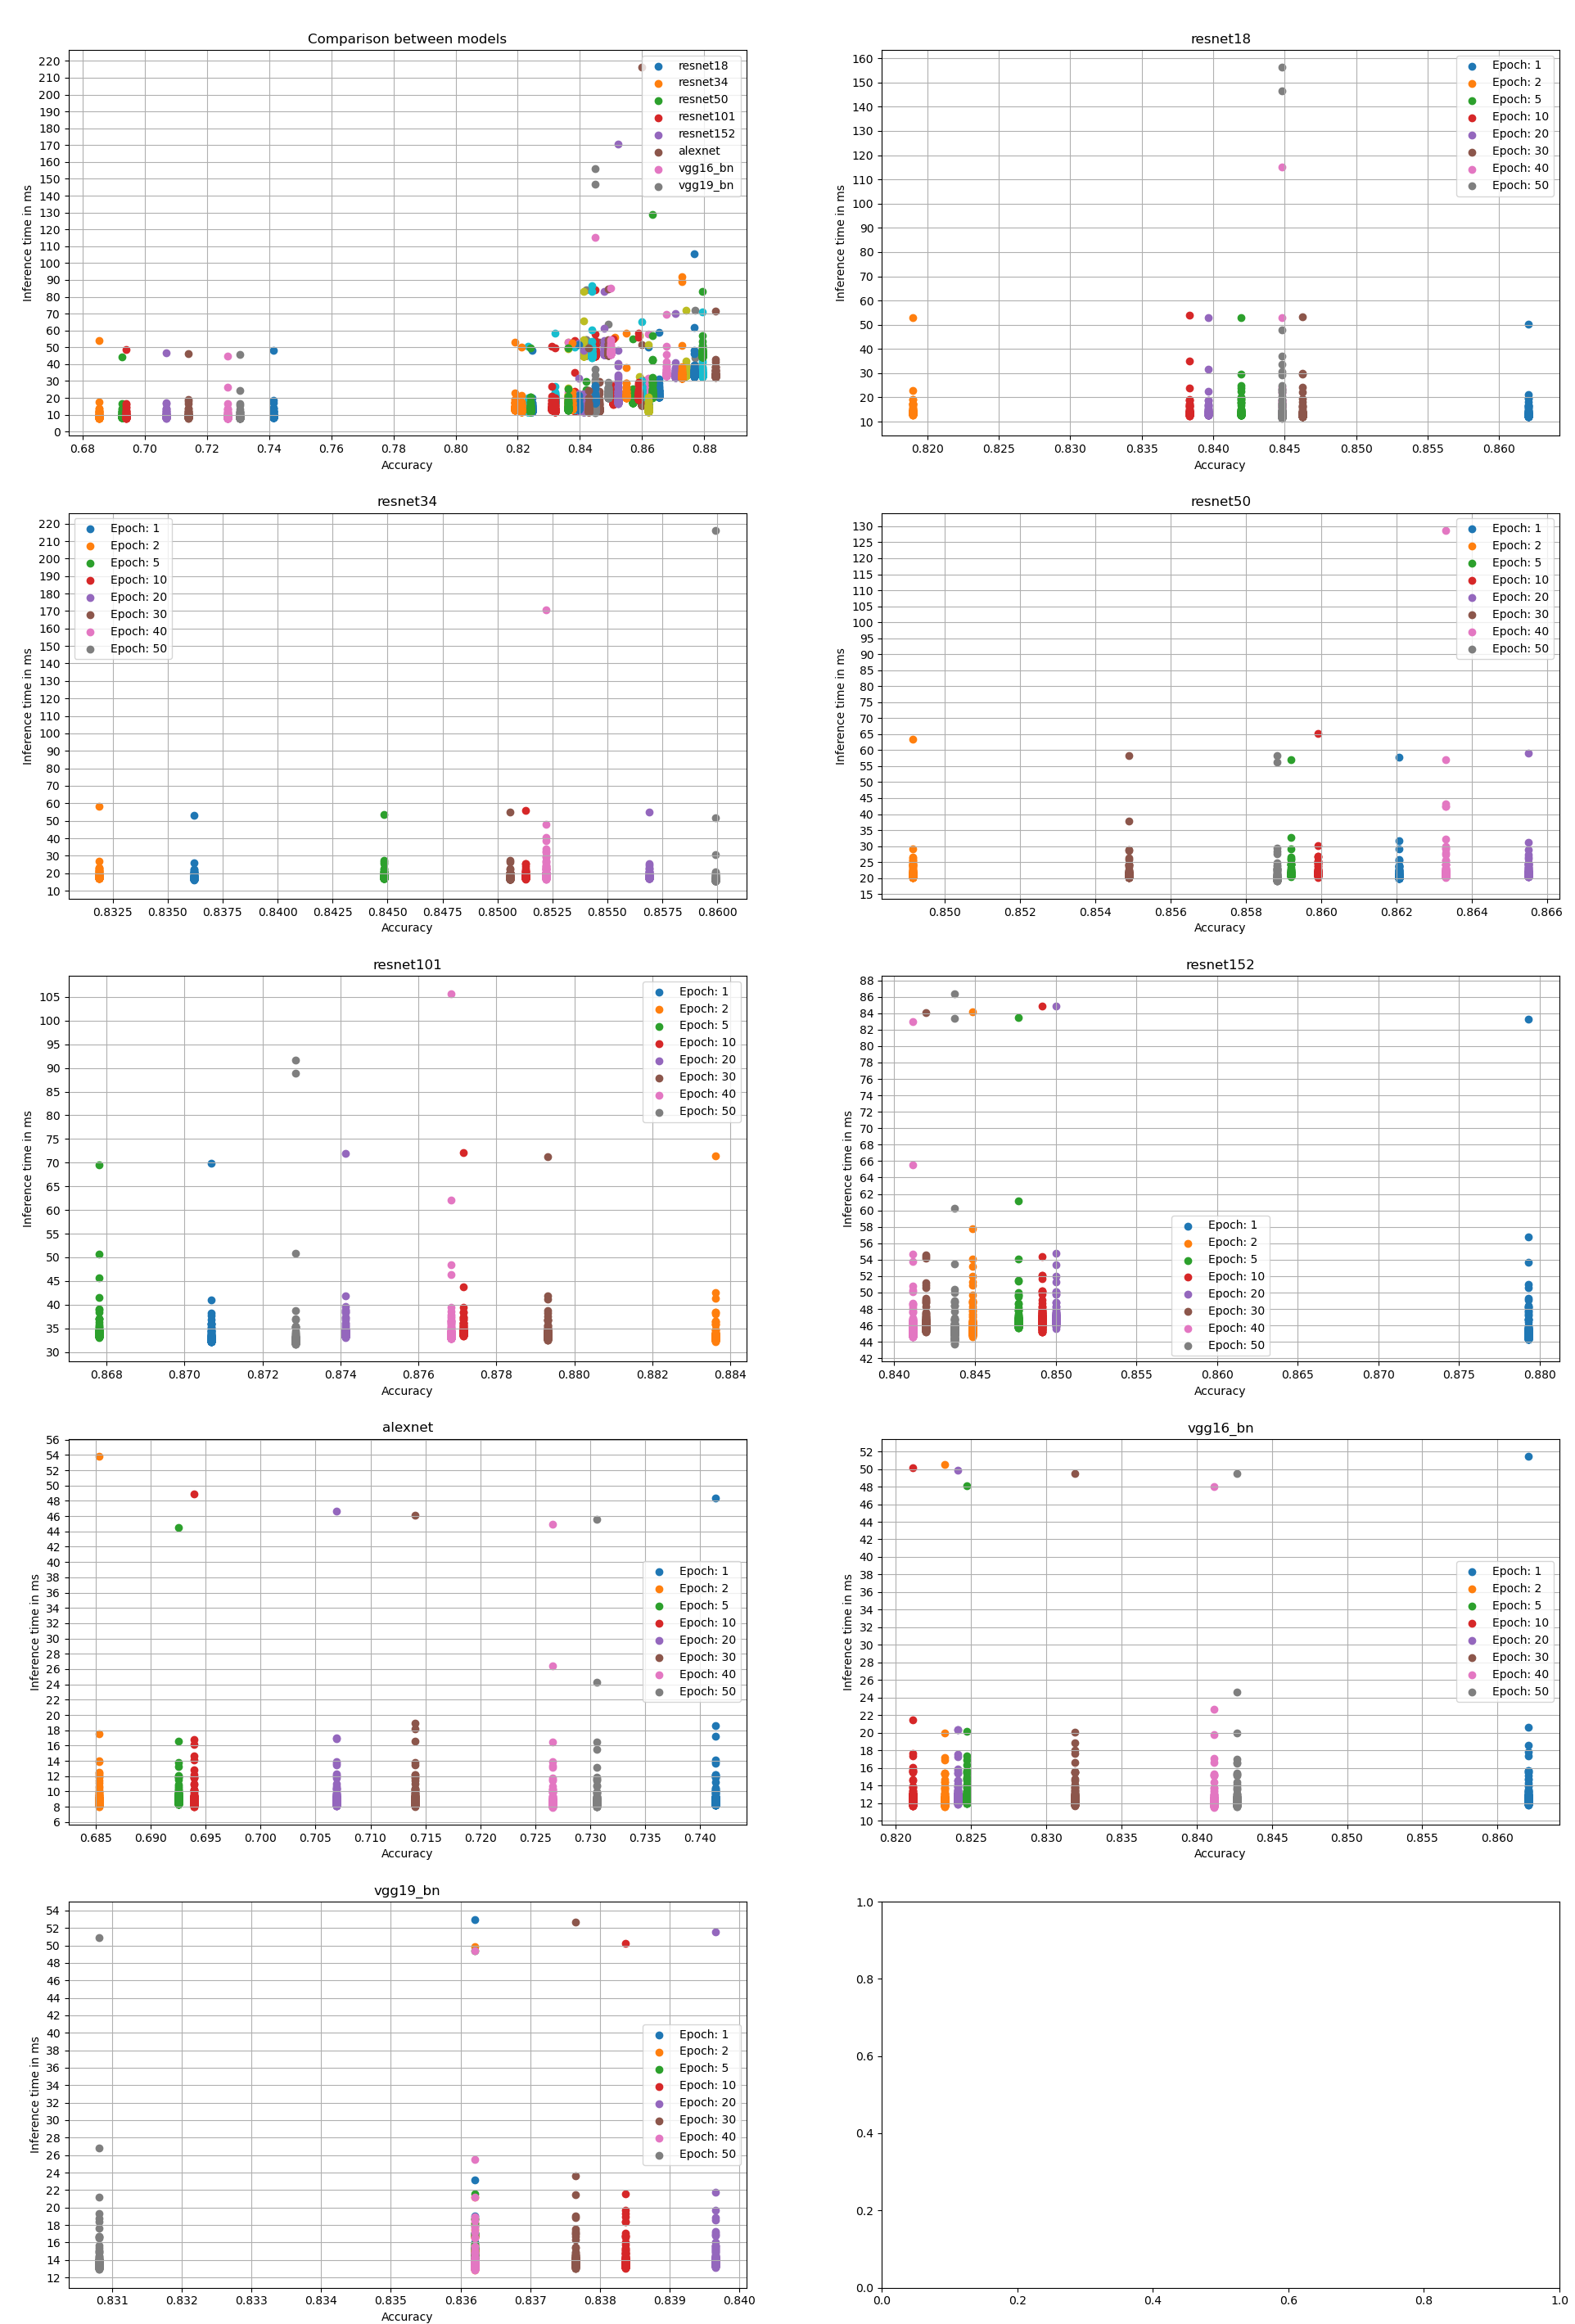
\includegraphics[width = 15 cm]{accuracy_inferencetime_seedlings_grey_train.png}
        \caption{Complete result of the test for inference time in the seedlings dataset with grey images}
         \label{fig:accuracy_inferencetime_seedlings_grey_train}
\end{figure}

\begin{figure}[ht]
       \centering 
	    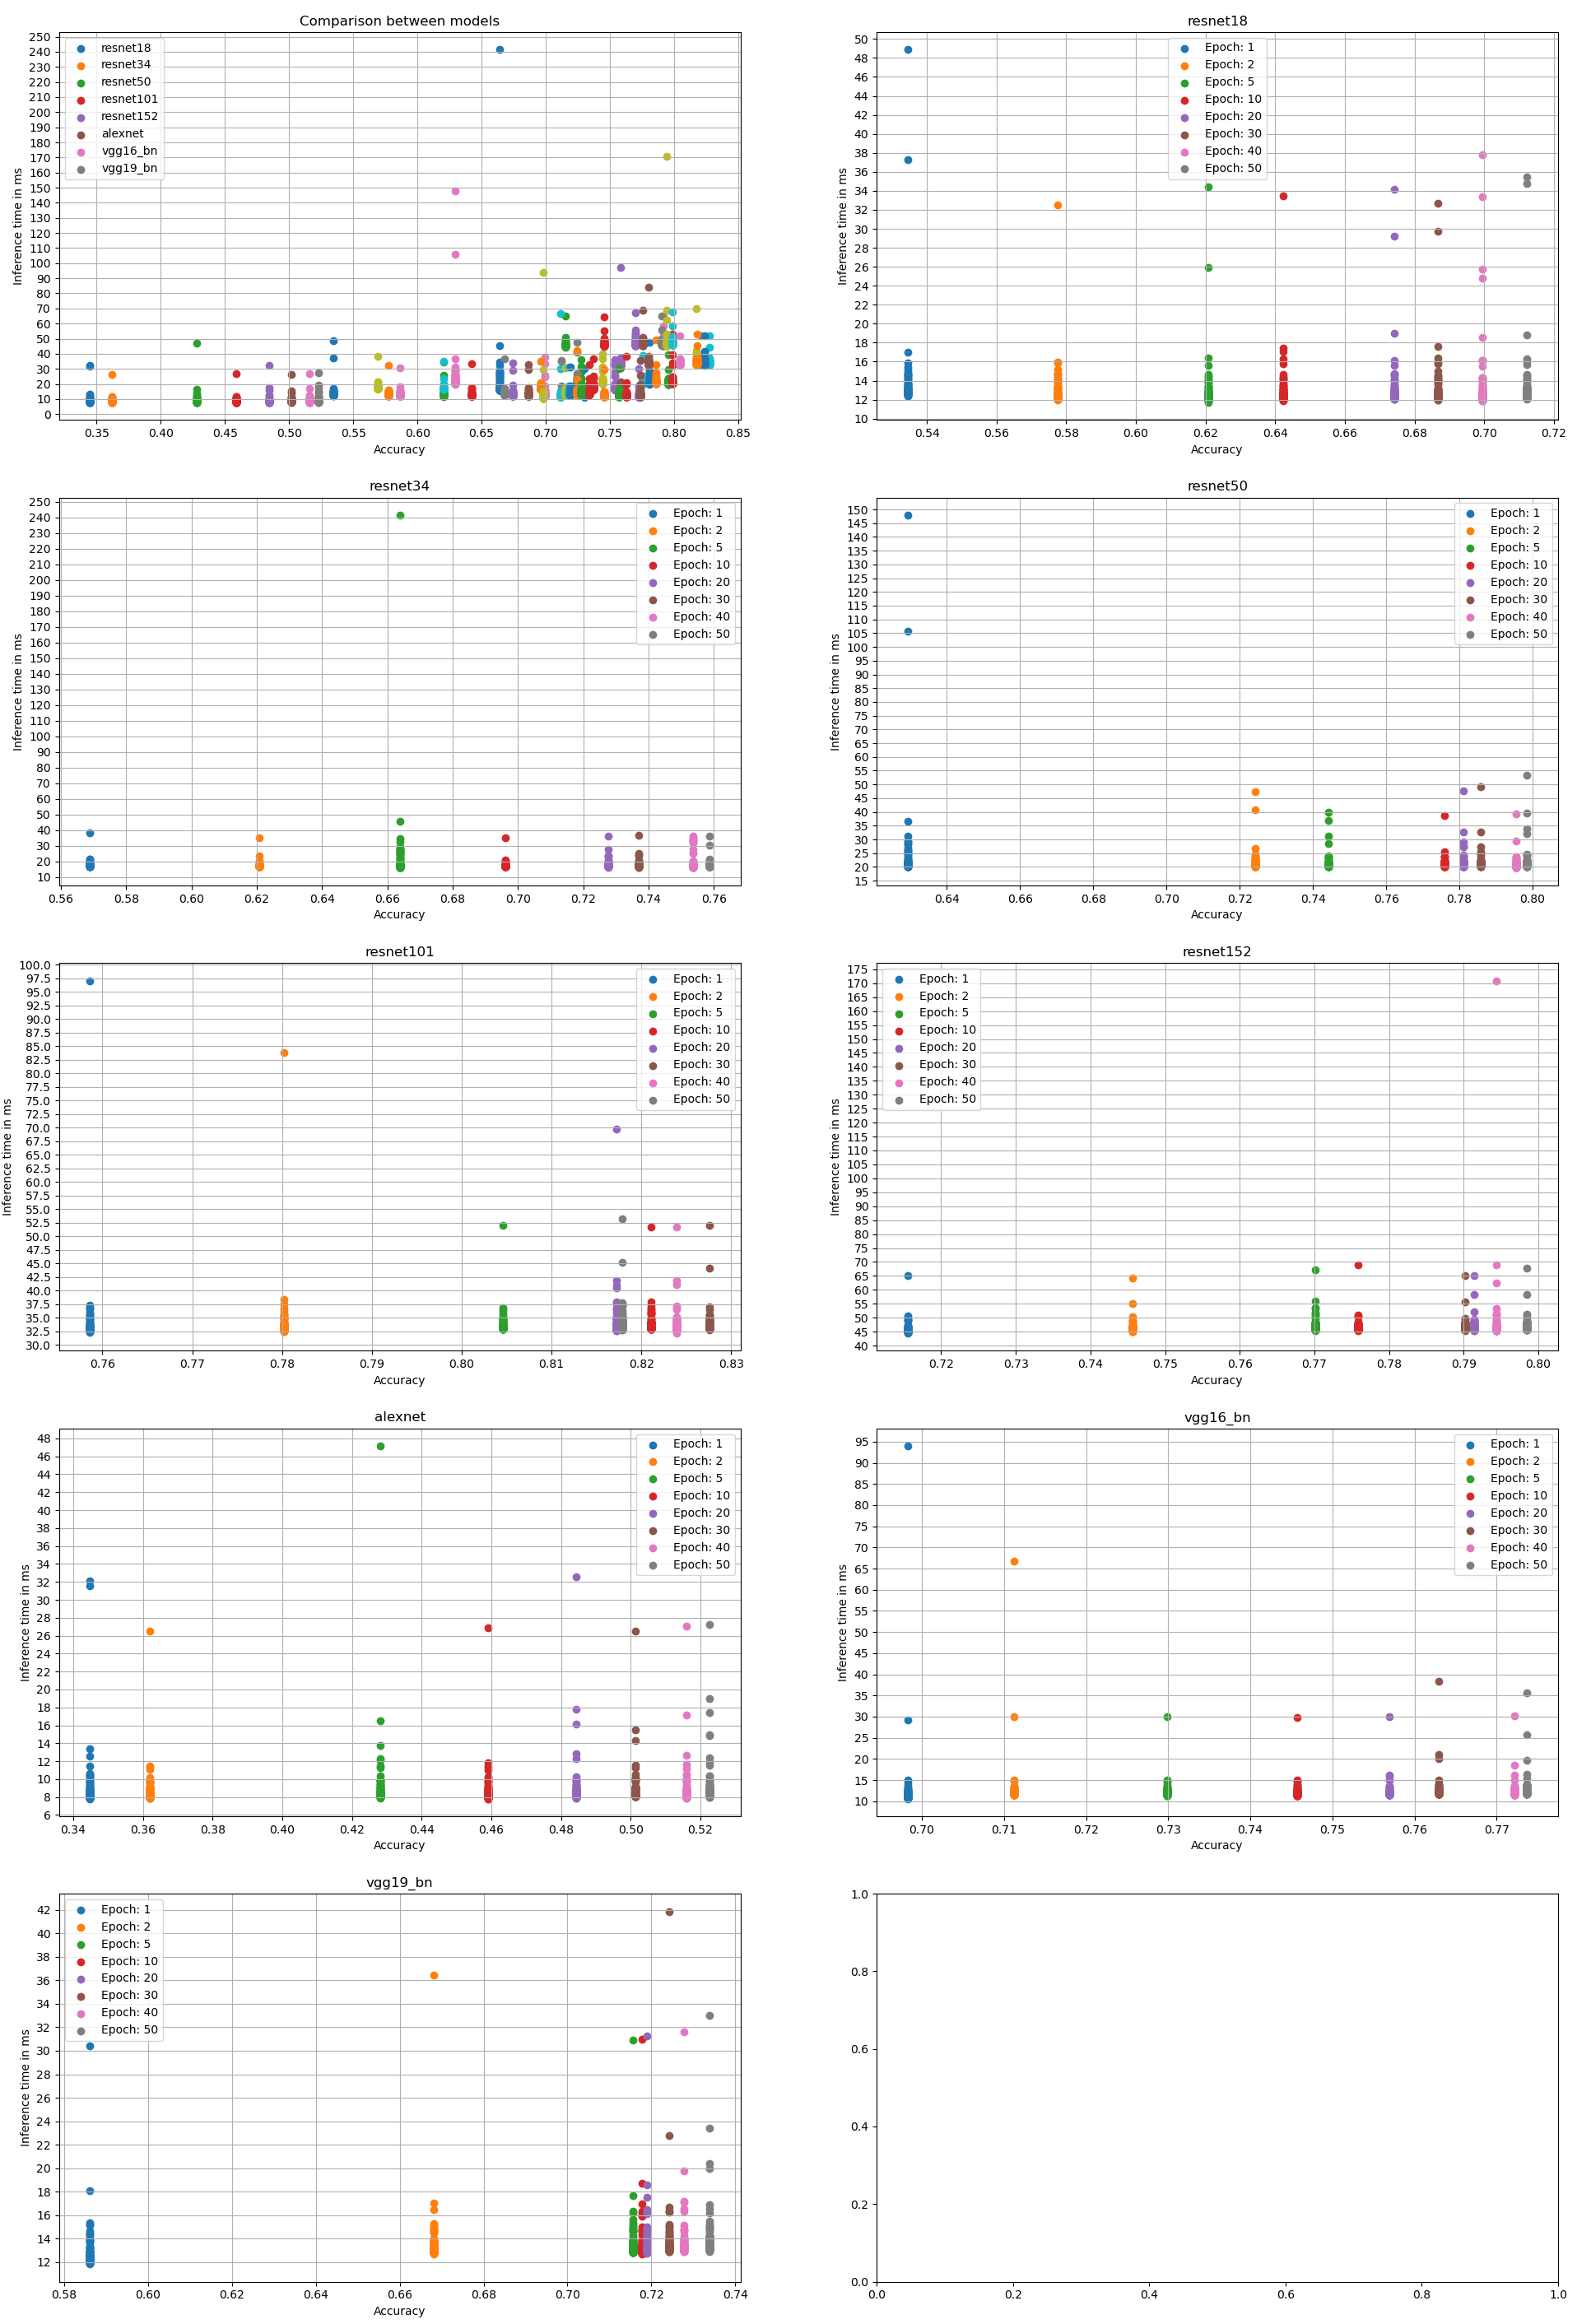
\includegraphics[width = 15 cm]{accuracy_inferencetime_seeds_grey.png}
        \caption{Complete result of the test for inference time in the seedlings dataset with grey images. The inference here is calculated by feeding grey scale images to the models}
         \label{fig:accuracy_inferencetime_seeds_grey}
\end{figure}